\documentclass[12pt]{report}
\usepackage{amssymb}
\usepackage{multicol}
\usepackage{graphicx}
\usepackage{subfigure}
\usepackage{verbatim}

\usepackage[letterpaper,left=1cm,right=2cm, top=1.5cm,
bottom=1.5cm,head=0cm,foot=1cm]{geometry}

\parindent=0in


\newcommand{\m}{\mbox{ m }}
\newcommand{\kg}{\mbox{ kg }}
\newcommand{\s}{\mbox{ s }}
\newcommand{\ke}{\mbox{\small KE}}
\newcommand{\pe}{\mbox{\small PE}}


\newcommand{ \probDir}[1]{{ \bf\small #1 \mbox{  }}}

\newcommand{ \breakList}{\setcounter{saveenum}{\value{enumi}} \end{enumerate}}
\newcommand{ \contList}{\begin{enumerate} \setcounter{enumi}{\value{saveenum}}}

\newcounter{saveenum}

\def \wspace{5cm}

%%%%%%%%%%%%%%%%%%%%%%%%%%%%%%%%%%%%%%%%%
\begin{document}

{\bf{Honors Physics} \hfill {Test: Momentum and Kinetic Energy} \hfill {Mr. Kelley}} \\ \\
%%%%%%%%%%
$\rho=mv$ \hfill $\ke=\frac{1}{2}mv^2$ \hfill $\pe=mgh$ \hfill $\rho_\circ = \rho_f$ \hfill $\ke_\circ + \pe_\circ = \ke_f + \pe_f$


\begin{enumerate}
\item How fast is a Steinway Model D Grand Piano (990 lb) moving when it hits the ground from the $3^{\mbox{\tiny rd}}$ floor (8.0 m)?  How fast is a banana (125 g) moving if it falls from the third floor?
\vspace{5cm}
\begin{itemize}
\item What is the maximum kinetic energy of the piano?  (2.2 lb = 1 kg)
\vspace{3cm}
\item What is the maximum kinetic energy of the banana?
\vspace{3cm}
\end{itemize} 

\item A 2 kg piece of clay hits a 2.5 kg piece of iron in outer space.  If the clay was traveling at 16 m/s with respect to the iron:
\begin{enumerate}
\item What will the final velocity be if the two objects stick together?
\pagebreak
\item What is the initial kinetic energy of the system?
\vspace{3cm}
\item What is the final kinetic energy of the system?
\vspace{3cm}
\end{enumerate}

\item A 160 g billiard ball, with initial velocity 10 m/s, hits a 145 g baseball.  The billiard ball deflects at an angle of $15^\circ$ at 8 m/s.  What is the magnitude and direction of the baseball's velocity?
\pagebreak

\item  Find the velocity of the ball on this frictionless track at points 1 and 2. \\ \\
{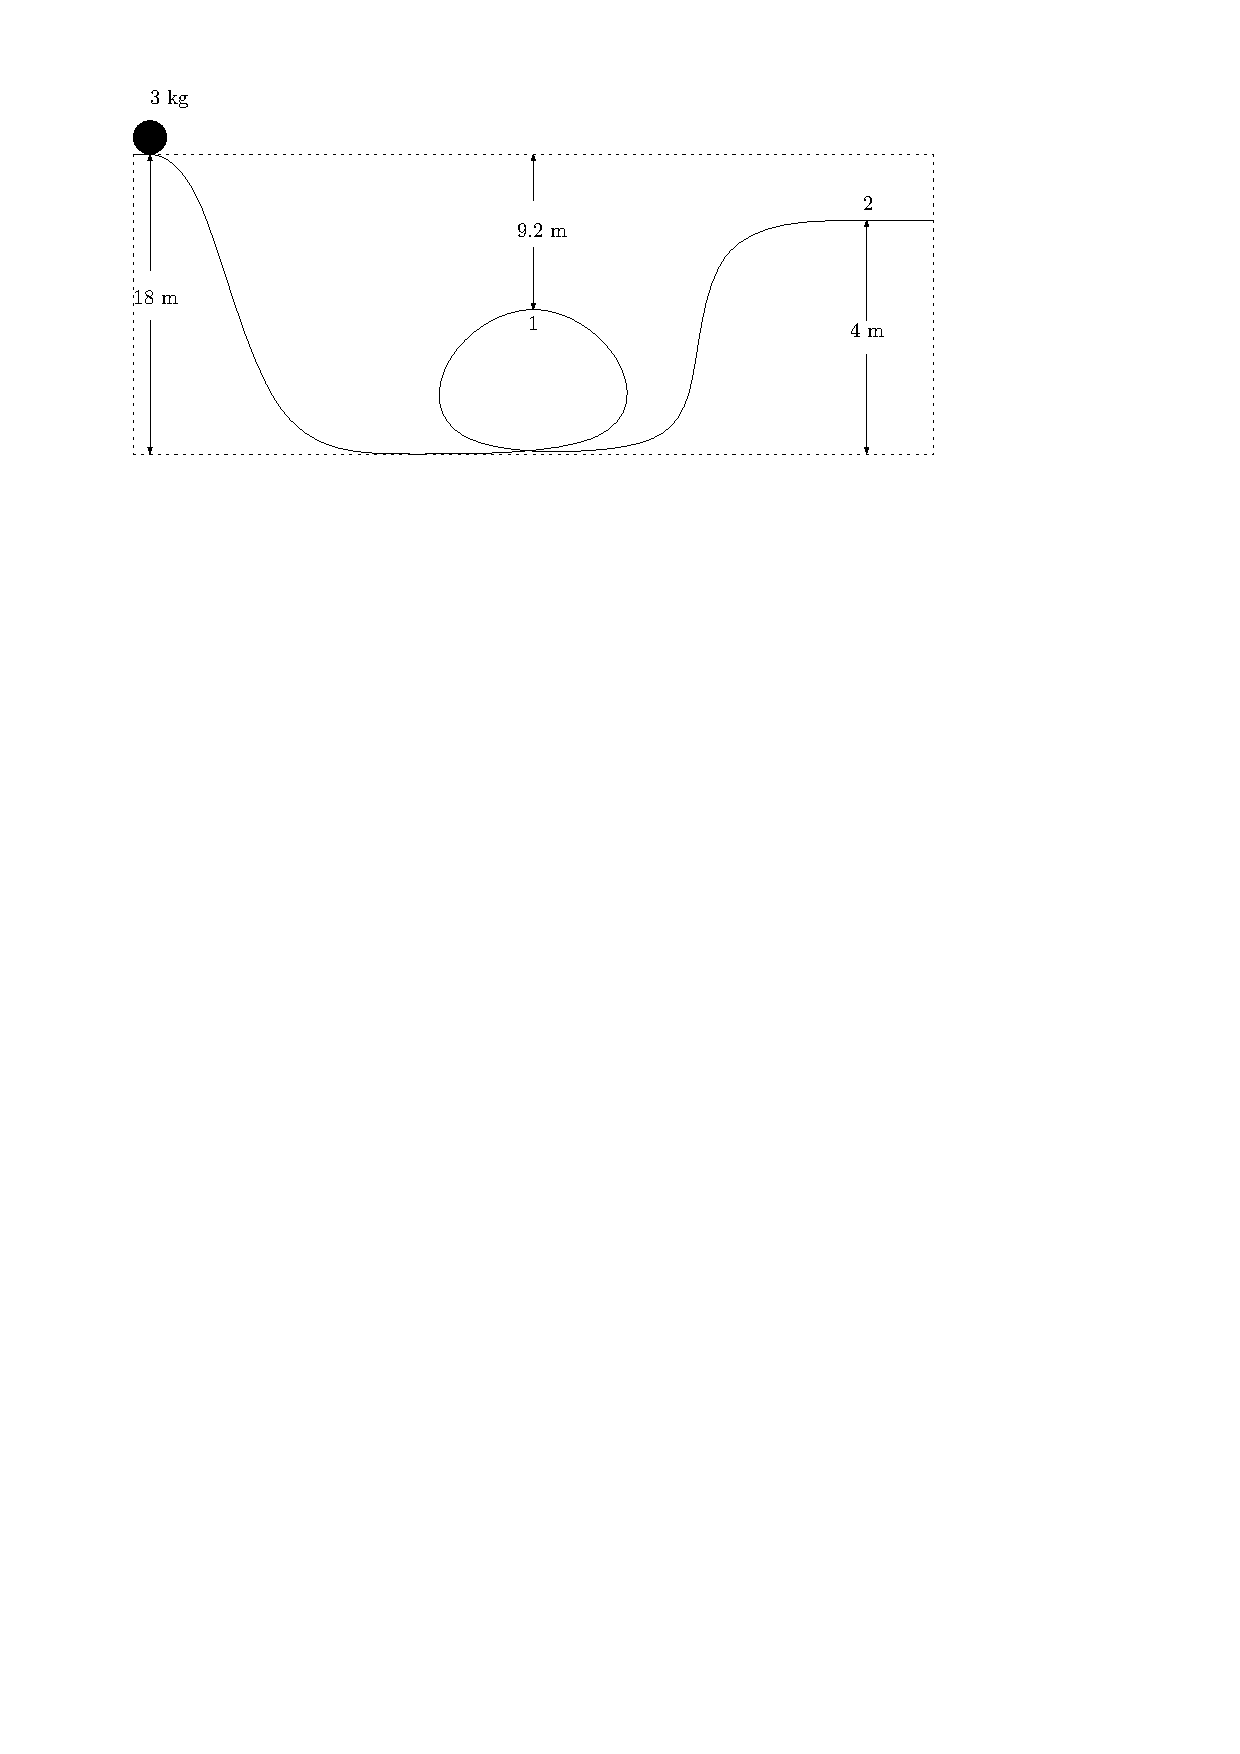
\includegraphics{energyCoasterLoop}}
\vspace{5cm}

\item A tennis ball hits a duck head-on.  The duck was flying with a speed of 5 m/s, and the tennis ball was traveling with a speed of 18 m/s.  If the tennis ball bounces straight back (reverses direction) with a speed of 4 m/s, how fast is the duck now going?  The duck has a mass of 1 kg and the tennis ball 57 g.  (Hint: UNITS! SIGNS!)
\pagebreak

\item Little Sally is on a collision course with a wall.  Her tricycle is out of control and she can't hit the brakes.  The wall is 2 meters wide.  Superman knows he can reach her when she is 1 m away from the wall.  If he catches her while flying perpendicular to her motion, how fast should he be going to \emph{just} miss the wall? \\ \\
Sally's mass and velocity are $m_s = 20\kg$ and $v_s = 3.5 \mbox{ m/s}$.  Superman's mass is 75 kg.  Draw Superman in the figure, and the desired path of Sally/Superman. \\ \\
Hint: $\tan^{-1}(\frac{y}{x}) = \theta \Longleftrightarrow \frac{y}{x} = \tan(\theta)$ \hfill{} \raisebox{-10cm}{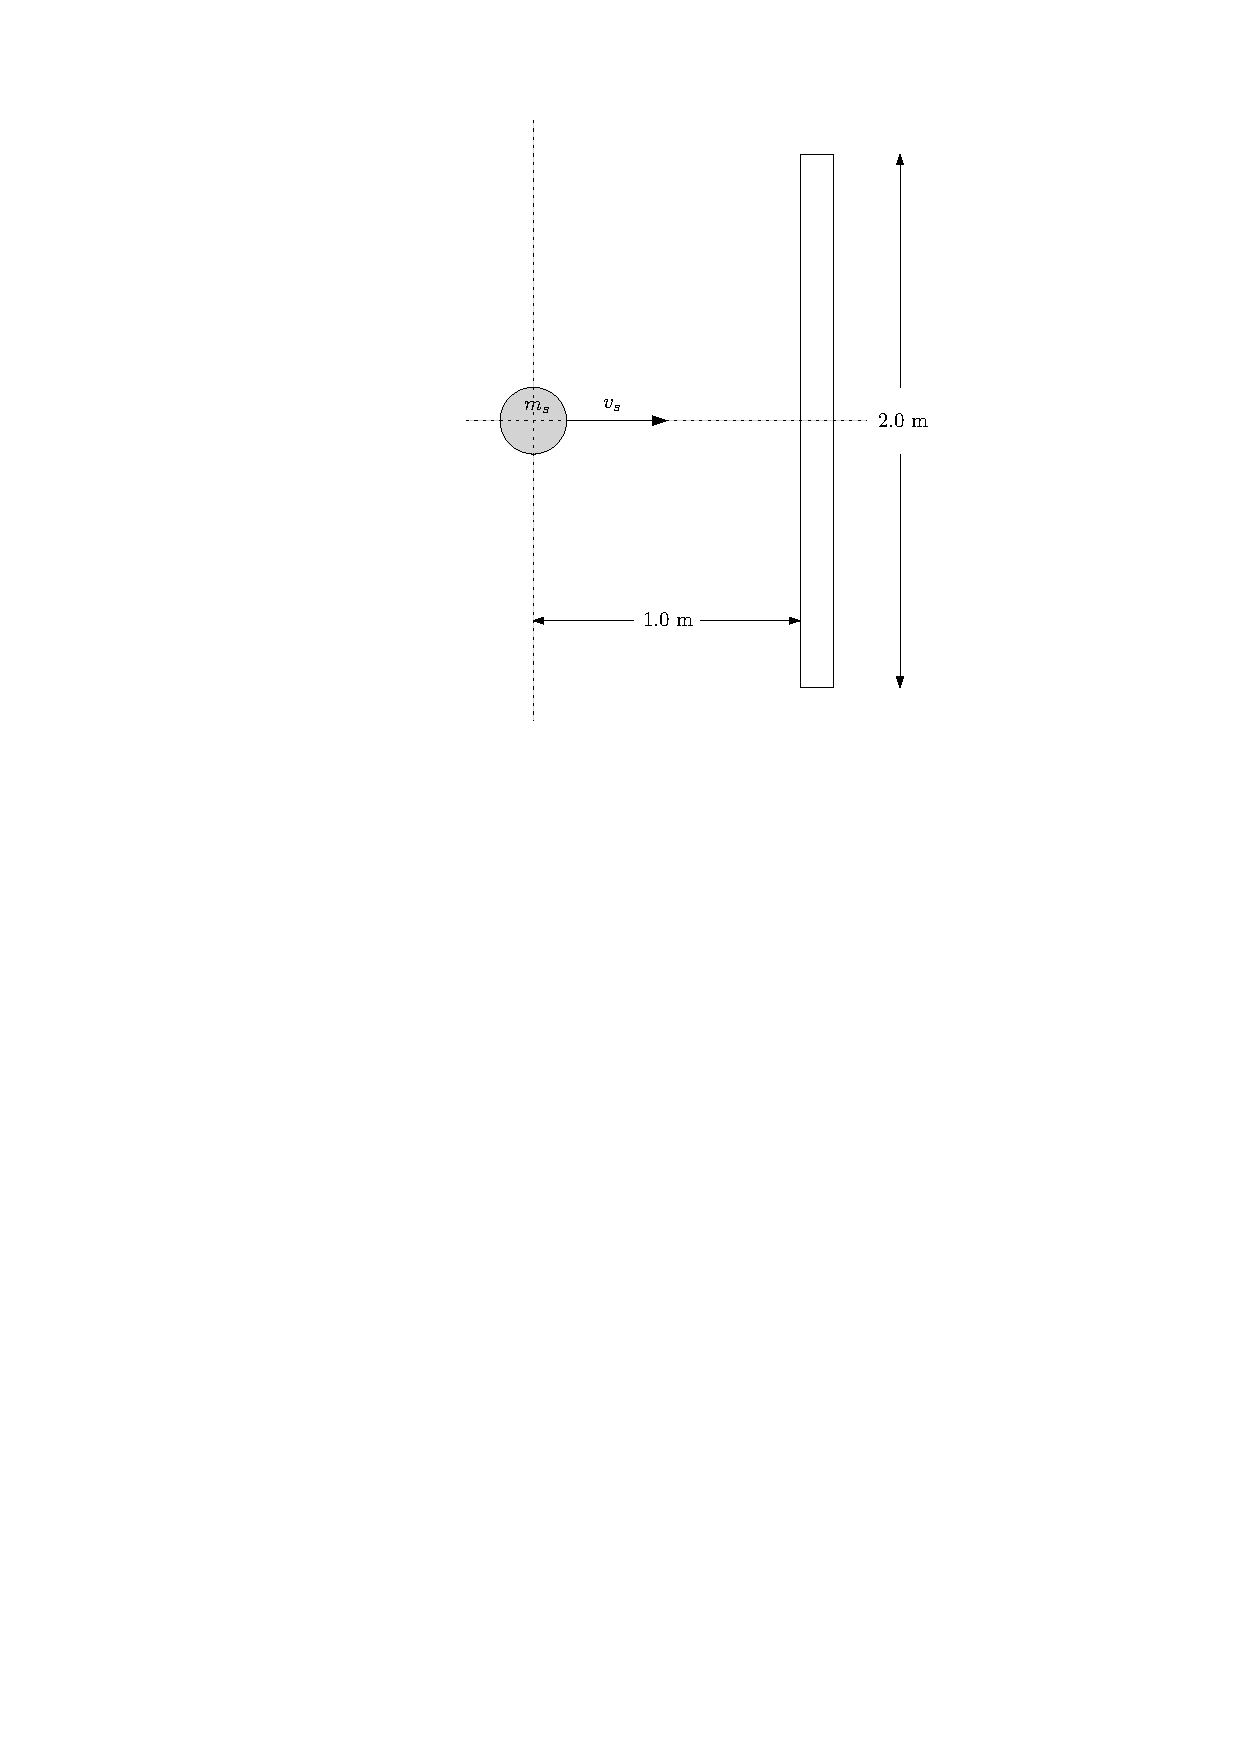
\includegraphics[scale = 1]{sallySuperman}}


\end{enumerate}




\end{document}